\documentclass[a4paper,12pt]{article}
\usepackage[utf8]{inputenc}
\usepackage{fullpage}
\usepackage[style=phys,maxbibnames=6]{biblatex}
\usepackage[skip=0.3em,indent=2em]{parskip}
\usepackage[pdftex]{graphicx}
\usepackage{float}
\usepackage{caption}
\usepackage{subcaption}
\usepackage{hyperref}
\usepackage{physics}
\usepackage{amsmath}
\usepackage{siunitx}
\usepackage{cleveref}
\usepackage{duckuments}


\addbibresource{references.bib}

\newcommand{\efn}{e4$\nu$}
\newcommand{\eGEN}{$e\text{-GENIE}$}

\newcommand{\verbb}[1]{\text{\verb|#1}}

\newcommand{\Mu}{$\mu$}
\newcommand{\Tau}{$\tau$}

\newcommand{\Ne}{$\nu_e$}
\newcommand{\Nm}{$\nu_\mu$}
\newcommand{\Nt}{$\nu_\tau$}

\newcommand{\Zz}{$Z^0$}
\newcommand{\Wp}{$W^+$}
\newcommand{\Wm}{$W^-$}
\newcommand{\Wpm}{$W^\pm$}
\newcommand{\pip}{$\pi^+$}
\newcommand{\pim}{$\pi^-$}

\newcommand{\duckim}[2][0.8]{
    \begin{figure}[h]
        \centering
        \includegraphics[width=#1\textwidth]{example-image-duck}
        \caption{
            Ducky: #2
        }\label{fig:nu_fen}
    \end{figure}
}


\begin{document}
\pagestyle{empty}
\par\noindent
\includegraphics[width=12cm]{PandA_crest.pdf}
\par\noindent

\vspace*{2cm}

\begin{center}
        \Large\bf \Large\bf Senior Honours Project \\
        \LARGE\bf Further analysis of \efn\ data
\end{center}

\vspace*{0.5cm}

\begin{center}
        \bf Jan Kocka \\
        February 2022
\end{center}
\vspace*{5mm}

\begin{abstract}
    In this project we continue the work on data from \efn.
    We further inspect the data generated with GENIE, mainly looking at the events producing 1 pion and comparing then to data from the CLAS experiment.
\end{abstract}

\vspace*{1cm}

\subsubsection*{Declaration}

\begin{quotation}
  I declare that this project and report is my own work.
\end{quotation}

\vspace*{2cm}
Signature:\hspace*{8cm}Date:  31/10/2021

\vfill
{\bf Supervisor:} Dr. Cheryl Patrick
\hfill
10 Weeks
\newpage

\tableofcontents

\newpage

\pagestyle{plain}
\setcounter{page}{1}

\section{Motivation and Background}
This project concerns neutrinos and their properties, and so a brief description of the relevant properties and their scientific significance is presented.
Neutrinos are 3 uncharged leptons of different flavours (each corresponding to the other 3, charged, leptons -- electron, \Mu\ and \Tau\ of ascending masses).
Neutrinos interact only via the weak force and with very low cross sections, the Feynman diagrams of their interactions with the other fundamental particles through the W and Z bosons are shown in \cref{fig:nu_feyn}.

Their existence was originally proposed by Pauli in the 1930s to explain the beta decay, and their mass was long thought to be 0, most notably the standard model assumes this.
However at the end of the last century neutrinos have been observed to undergo oscillations which implies non-zero mass.
Since then they have been at the forefront of research, nowadays they are accepted to have mass and there are questions about them being their own antiparticles (Majorana) and possibly violating charge-parity symmetry.
The answers to these questions could significantly further our understanding of the universe, including explaining the dominance of matter over antimatter.

\begin{figure}[h]
    \centering
    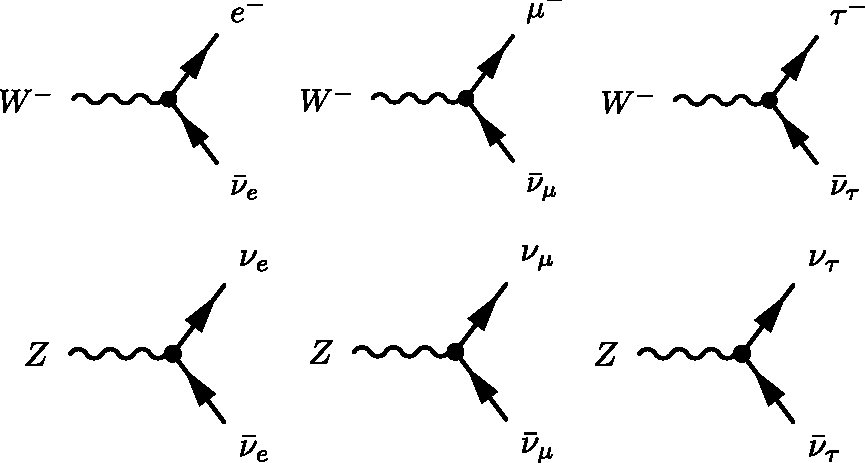
\includegraphics{figures/NeutrinoFeynman.pdf}
    \caption{
        Feynman diagrams of weak force vertices for neutrino interactions, all other vertices including them can be obtain by suitable rotations of these
        (this requires replacing some particles with their antiparticles, including the \Wm becoming a \Wp).
        Say the first could be changed to represent a $e^-$ and \Wp\ colliding and forming a \Ne.
        Figures taken from \cite{potterFeynmanDiagramsParticlea}.
    }\label{fig:nu_feyn}
\end{figure}

\subsection{Neutrino Oscillations}
In particle physics oscillations is a phenomenon that takes place when the particle mass eigenstates which govern its evolution in time are not the same as the state in which it is observed.
This phenomenon is not exclusive to neutrinos, the neutral Kaon has been known to oscillate to its own antiparticle and vice-versa since before neutrino oscillations were discovered \cite{burkhardtWavelengthNeutrinoNeutral2003}.
% However it might seem a bit abstract, but as we know from basic quantum mechanics when we make an observation, the observed system will collapse into some particular state depending on the result of our observation.

In the case of neutrinos, we say there are 3 flavours and the way we differentiate them is by the weak interaction, as so far all interactions we observed conserve the 3 separated lepton numbers (electron, \Mu\ and \Tau\ again).
So say an electron capture takes place when an electron interacts with a proton to form a neutron and a neutrino, then we observe that neutrino to be an electron neutrino in order to conserve the electron lepton number and we can say it is collapsed into the electron neutrino eigenstate.

Further, that electron eigenstate can be expressed in terms of the mass eigenstates, and if the 2 eigenstate sets aren't identical it will have multiple non-zero components.
Then as the mass eigenstates travel differently (the neutrino has a definite $E$ and so through $E^2 = m^2 + p^2$ we get that the mass eigenstates have different momenta and so speeds), the relative components of the state at different positions as it travels will change periodically -- oscillate.
Thus the probabilities of measuring the neutrino in any of the 3 flavour states also oscillates.
% The result is that if a neutrino is measured to be of some known flavour the probability of measuring it at a later time in any of the other flavour states changes and it might later be measured to be of a different flavour.

A very important property resulting from the two eigenstate sets being different is the transformation matrix between them.
For neutrinos this is the PMNS\footnotemark\ matrix, it is referred to as $U$ and is such that 
\begin{equation}
    \ket{\nu_\alpha} = \sum_i U_{\alpha i} \ket{\nu_i}, \text{ and }
    \ket{\nu_i} = \sum_\alpha U^\dag_{i \alpha} \ket{\nu_\alpha}
\end{equation}
where $\ket{\nu_\alpha}$ are the 3 flavour eigenstates and $\ket{\nu_i}$ the mass eigenstates.
The exact form of the matrix then determines many of the neutrino properties, obtaining accurate values for its elements is the main driving force of neutrino oscillation experiments.
For example if the matrix is not completely real then neutrinos violate CP symmetry.
\footnotetext{Stands for Pontecorvo–Maki–Nakagawa–Sakata matrix, it is the analogue of the CKM matrix for the mixing of quarks.}

Then to complete the picture, the probability of a neutrino measured to be of flavour $\alpha$, to be measured again in the flavour $\beta$ is given by 
\begin{equation} \label{eq:nosc}
    P(\alpha \rightarrow \beta) = \sum_i |U_{\alpha i} U^\dag_{i \beta}|^2 + 2\Re \sum_{j>i} U_{\alpha i} U^\dag_{i \beta} (U_{\alpha j} U^\dag_{j \beta})^* \exp(-i\frac{\Delta m^2_{ij}}{2}\frac{L}{E})
\end{equation}
where $E$ is it's energy, $L$ the distance between our measurements and $\Delta m^2_{ij}$ the mass difference of the mass eigenstates $i, j$ squared (for more detail see \cite{zuberNeutrinoPhysics2020}).
This is then our main entry point for studying the PMNS matrix from oscillation experiments as we can measure these probabilities $P$ and deduce some of the values or their relations along with the mass differences $\Delta m_{ij}$.
Though even if we  knew precisely all the oscillation probabilities we still can not fully determine the matrix, there may be a Majorana phase component that doesn't influence $P$ and so needs to be studied using other experiments.

\subsection{Oscillation Experiments and Energy Reconstruction}\label{sec:exanderec}
There are active experiments (NOvA and T2K currently running and DUNE and Hyper-Kamiokande under development) working on precise neutrino oscillation measurements to determine the neutrino masses and PMNS matrix elements.
% There are active experiments (including Super-Kamiokande, OPERA, MINOS, DUNE and Hyper-Kamiokande\footnote{**maybe change which ones I mention and add references to them}) working on precise neutrino oscillation measurements to determine the neutrino masses and PMNS matrix elements.
In all of these experiments neutrinos from a source which has known fractions of the 3 flavours are beamed across large distances (for oscillations of 1\si{GeV} \Nm\ an $L$ of order $\sim 1000\si{km}$ is needed \cite{mezzettoThreeFlavorOscillationsAccelerator2020}) so that they oscillate and then some of the flavours (electron, \Mu\ or both) are observed and counted.
This means we are measuring some of the probabilities from \cref{eq:nosc} with a known $L$, however we don't have a simple value for $E$ which we need in order to interpret the data.
Experiments typically use either neutrinos from the sun, from the atmosphere due to the cosmic microwave background or from secondary neutrino beams at accelerators and all of these methods produce neutrinos with wide ranges of energies.
Because of that experiments rely on reconstructing incident neutrino energies and for that a very good understanding of the detecting mechanism is needed.

\begin{figure}[h]
    \centering
    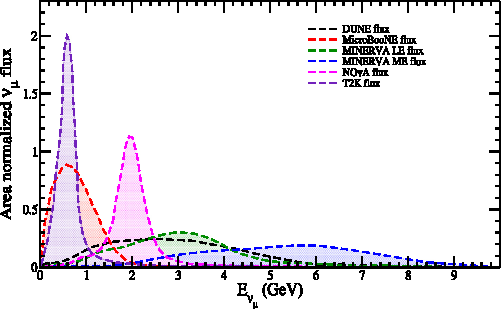
\includegraphics[width=0.6\textwidth]{figures/sourceEnergies.pdf}
    \caption{
        The energy distributions of neutrino sources used at various experiments.
        All of these are accelerator based sources which have the narrowest energy distributions, however still the spread is on the order of hundreds of \si{MeV}.
        Figure taken from \cite{sajjadatharNeutrinosTheirInteractions2023}.
    }
\end{figure}

As neutrinos are uncharged and have tiny cross sections, they aren't detected directly, instead a large amount (needed due to the small cross sections) of some stable substance (argon, water or chlorine) is stored and surrounded by detectors (often carbon based scintillators).
Then when neutrinos come in, some will interact with these atoms and produce detectable particles.
These always have to include a lepton of the corresponding flavour and possibly other particles, often pions, nucleons or photons and a collection of particle measurements originating from one neutrino is called an event
While the neutrinos can interact with the atomic electrons \cite{whittinghamScatteringLowEnergy2022}, it is only significant at low neutrino energies and rarely relevant to oscillation experiments.
Thus some of the most important physics of neutrino detectors are the neutrino-nucleus interactions and these are not yet well understood.
Modern oscillation experiments report the model limitations to be a source of large systematic uncertainties\cite{abeConstraintMatterAntimatter2020,novacollaborationNewConstraintsOscillation2018}.

Which is where \efn\ comes in, while ideally we would study these interaction with neutrinos, the absence of a monoenergetic neutrino source, along with other complications (CITATION) makes us consider other options.
While on the surface they seem different, electrons scatter off of nuclei in a similar manner, further after the first neutrino-nucleus interactions, the resulting hadrons will often interact with each other too.
This is called Final State Interactions (FSI) or nuclear effects, these are very relevant to oscillation experiments and identical for neutrino and electron-nucleus scattering.
So in summary, we can use easily available electron scattering data to test neutrino interaction models -- \efn.

% in order to better interpret data from neutrino detectors and mainly to improve their energy reconstruction (which is becoming a significant factor on the uncertainties of the results) we need to understand these neutrino-nucleus interactions better.

% However, as there are no monoenergetic neutrino beams it is very difficult to experimentally study these effects directly on neutrinos, so instead we study electron-nucleus interactions which are subject to the same quantum field theory interactions.

\subsection{Neutrino(Electron)-nucleus interactions}
As the interactions are not yet fully, fundamentally understood, we to a large degree resort to classifications which allows us to make prediction under certain conditions.
Firstly, both neutrino and electron nucleus scattering can be described by
\begin{equation}
    l + A \rightarrow l' + a + b + c ...
\end{equation}
where an incoming lepton $l$ scatters off of a nucleus $A$ resulting in a lepton $l'$ and hadron particles $a, b, c ...$.
When considering realistic experiments we always know $l$ and $A$ but might only be able to detect the outgoing lepton and some or none of the outgoing hadrons. 
To differentiate these cases we consider separately \emph{inclusive} cross sections where only $l'$ is detected (so the result is essentially as if summing over all the possible outgoing hadrons).
\emph{Semi-inclusive} cross sections where $l'$ and some of the hadrons are detected and \emph{exclusive} cross sections where we know all of the resulting particles \cite{amaroElectronNeutrinonucleusScattering2020}.

As neutrinos only interact via the weak force, all neutrino-nucleus interactions take place via either the \Zz\ boson, in which case the final lepton is the same neutrino and so these events are not detected.
These are called \emph{Neutral Current} (NC) events and are generally difficult to measure as we cannot measure the outgoing lepton and have to rely on reconstructing the event solely from the hadrons \cite{giustiNeutralCurrentNeutrinonucleus2020}.
Or it can interact through the \Wp and \Wm\ bosons (\emph{Charged Current} or CC interactions) in which case a charged lepton is produced and detected, often being the most important particle for detection and event reconstruction.

This is contrasted to electrons which will dominantly interact with the nucleus through photons (so preserving the electron).
Nevertheless within quantum field theory the neutrino weak force interactions have a vector and an axial-vector components and the electron EM interaction has only a vector component\cite{alvarez-rusoNuSTEC11NeutrinoScattering2018}.
Thus, the vector part of neutrino-nucleus scattering calculations and simulations can be adapted and tested by electron scattering.

\subsubsection{Event kinematics}

% Due to this existing MC event generators like GENIE can be modified to generate electron-nucleus interaction events and test particularly the vector current component of the theories behind the generator.
% Further on I will only speak about neutrino interactions, but most of these characteristics apply to electrons too.

\begin{figure}[h]
    \centering
    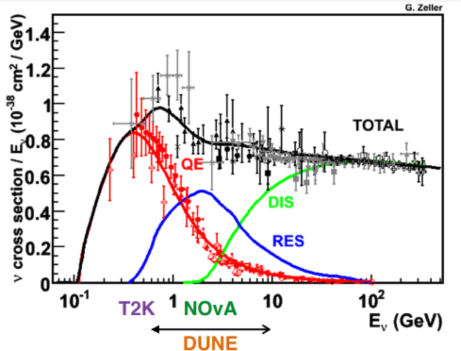
\includegraphics[width=0.6\textwidth]{figures/sigmaVsEnu.pdf}
    \caption{
        Replace this with a better image and a source!!
    }\label{fig:nusigma_vs_Enu}
\end{figure}

Finally to come back to the interaction types mentioned in \cref{sec:exanderec}, the main types relevant for oscillation experiments are Quasi-Elastic (QE), Resonant (RES) and Deep Inelastic Scattering (DIS).
In this order these dominate at increasing energies (see \cref{fig:nusigma_vs_Enu}), a low energy neutrino ($<1\si{GeV}$) will essentially bounce off of a nucleus/a single nucleon from it as a whole.
At medium energies ($\sim 1 \si{GeV}$) the neutrino can excite a nucleon into an excited state and at the highest energies ($>3\si{GeV}$) the neutrino will interact with many particles and DIS interactions become difficult to predict especially once accounting for FSI.

\subsubsection{Quasi-Elastic (QE) scattering}
Elastic scattering refers to processes where the internal structure of the colliding objects isn't altered.
Naturally then, fully elastic neutrino scattering can only happen within NC interactions.
However, there is a very similar type of CC interaction where the neutrino interacts interacts with the nucleus, mostly as a whole, but converting one of the neutrons to a protons, shown in \cref{fig:QE_fd} (a similar process for an antineutrino would convert a proton into a neutron), these are QE interactions.
As mentioned before, these dominate at lower neutrino energies and in many ways are the simplest interaction as don't need as much information about that nucleus.

\begin{figure}[h]
\centering
    \includegraphics[width=0.9\textwidth]{example-image-duck}
    \caption{
        Ducky: QE interaction Feynman diagram
    }\label{fig:QE_fd}
\end{figure}

Of the neutrino interactions, QE are the best theoretically understood, the simplest models rely on a combination of two independent parts: calculations of neutrino-nucleon interactions within the impulse-approximation and modelling of the nucleons within the nuclei.
A recent review \cite{gallagherNeutrinoNucleusInteractions2011} has compared the theoretical result with observations from the MiniBooNE and NOMAD.
While the models capture many important features, there are also significant discrepancies which point to the interaction being more complicated than thought and also points out that many studies consider different levels of inclusiveness leasing to difficulties in comparisons.

% I won't go into further detail as we don't examine them in this work (so they are just background that we try to eliminate) however it is worth noting that the elastic scattering of electrons off of nuclei 

As they are not a focus of this work, I won't go further into detail, however it is worth saying that QE interactions are also a great example of the similarities of neutrino and electron scattering.
The elastic electron scattering off of nuclei is closely related and in the two have often been studied together, also being the dominant interaction at lower energies.

\subsubsection{Resonant scattering}

\subsubsection{Deep Inelastic scattering (DIS)}

\subsection{The GENIE Event Generator \cite{andreopoulosGENIENeutrinoMonte2010}}
Due to the amount expertise required to understand either the theory or the experimental aspects of neutrino interactions, it becomes difficult to package theories in a way that they can be easily understood and tested by experiments.
The fact that recently the Neutrino Scattering Theory-Experiment Collaboration (NuSTEC \cite{alvarez-rusoNuSTEC11NeutrinoScattering2018}) has been started is a sign of this.
As a result, Monte Carlo (MC) neutrino event generators are often used to package theoretical models in a way that predictions can be made.
GENIE is the most widely adopted such MC generator, first released for use in 2007 it aims to be a canonical generator accurately reflecting the state-of-art theories for a wie range of energies and targets.
It is a large codebase of modern C\texttt{++} code using the popular ROOT libraries\cite{brunROOTObjectOriented1997} and is particularly well tuned to a tested on the few \si{GeV} energy neutrinos that are of interest to oscillation experiments.

As is described in \cite{andreopoulosGENIENeutrinoMonte2010}, there are 3 main categories of models in GENIE.
Nuclear physics models model the nuclei and their composition, this strongly depends on the energy of the incoming neutrino and whether it will scatter off of a whole nucleon or a quark.
GENIE uses a Relativistic Fermi Gas (RFG) model for this step which is particularly successful at lower energies.
Then cross sections are calculated for various scattering types using their cross-section models and one is randomly chosen according to these.
These types include the ones mentioned above, but they are both further divided ooterh interactions are considered, including NC scattering and neutrino-electron scattering.
Finally, hadronization models account for FSI, for these GENIE uses the AGKY model from the MINOS experiment \cite{HadronizationModelMINOS}.

GENIE also has an electron scattering mode (\eGEN) that has been revised in 2021 by the \efn collaboration \cite{e4ncollaborationInclusiveElectronScattering2021}.
This uses the same underlying logic and structures of GENIE to generate electron-nucleus scattering events, data from which has been in used in this report.

\section{The \efn\ Data}
The data used by the \efn\ analysis comes from the e2a experiment measuring electron scattering at electron energies of 1.159, 2.257 and 4.453 \si{GeV} on targets of He, C and Fe nuclei.
The measurements took place in Thomas Jefferson National Accelerator Facility (JLab) using the CEBAF Large Acceptance Spectrometer (CLAS6) \cite{meckingCEBAFLargeAcceptance2003} in 1999, the data has been used in many published works including \cite{khachatryanElectronbeamEnergyReconstruction2021}.
In addition, recently CLAS has undergone an upgrade (CLAS6 to CLAS12) \cite{burkertCLAS12SpectrometerJefferson2020} allowing experiments at electron energies up to 12 \si{GeV} and generally improved capabilities.
The \efn\ collaboration has a CLAS12 experiment under development, with new data starting at electron energies of $\sim6 \si{GeV}$ expected to be ready soon.
Along collection of measured events we also have a collection of GENIE generated events for the same energy and target (for the $\sim 2\si{GeV}$ neutrino energy C target we have 1 million measured and 175 million GENIE generated events).

These datasets are each in a ROOT file in a GENIE format called \verbb{gst}, this is a list-like object (\verbb{TTree}) of events with their properties.
As this is a GENIE format, there are fields for many properties not measured in experiments, for the CLAS6 data these are empty.
Some of the more notable fields are the outgoing electron 4 momentum, information about all the particles after the neutrino-nucleus interaction (referred to as primary or initial state) as well as the same information about post FSI particles (final state).
Some of these properties, especially the ones that never could be measured, are referred to as the `truth` as they reflect what we think is physically going on.
Finally, as the detector is not perfect there are many steps of adjusting the `truth` data before it can be compared to experiments, these are covered in detail later as they are a big part of this project.

\subsection{The CLAS detector}
The CLAS6 detector, active from 1998 to 2012 when the work on CLAS12 has began, is largely built around a set of 6 toroidal magnets distributed along the azimuthal angle $\phi$.
These curve the trajectories of charged particles in their $\phi$ plane and allow for charged particle momentum measurements in drift chambers.
They also give rise to distinct 6 sectors visible in \cref{fig:CLAS} and deadspace between them from particles hitting the magnets.

\begin{figure}[h]
    \centering
    \begin{subfigure}[b]{0.45\textwidth}
        \centering
        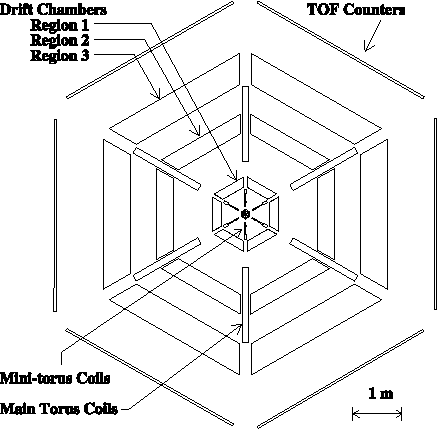
\includegraphics[width=\textwidth]{figures/CLAS_headon.pdf}
        \caption{CLAS6 as seen along the beam axis.}
    \end{subfigure}
    \hfill
    \begin{subfigure}[b]{0.5\textwidth}
        \centering
        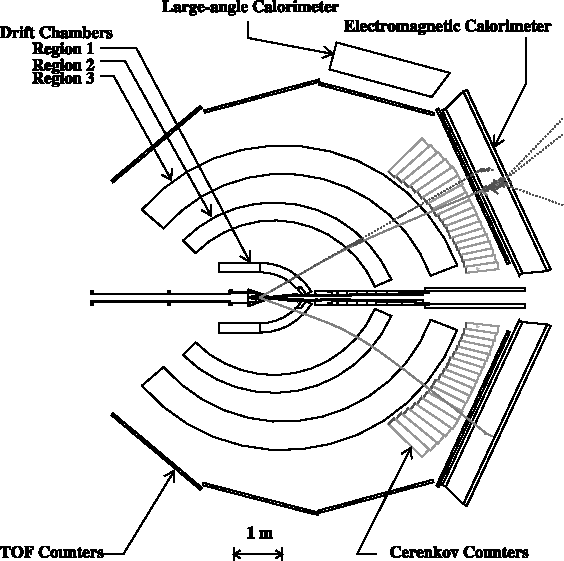
\includegraphics[width=\textwidth]{figures/CLAS_side.pdf}
        \caption{Side view cross section through the detector.}
    \end{subfigure}
    \caption{\label{fig:CLAS}
        Diagrams of the CLAS6 detector from \cite{meckingCEBAFLargeAcceptance2003}, see for more detail.
        Most important for us are the EM calorimeter spanning $\theta < 60$ which detects the scattered electrons and photons.
        Cherenkov counters near the axis are needed for distinguishing electrons and negative pions and the time-of-flight (TOF) detectors help distinguish protons and positive pions.
    }
\end{figure}

Our data, from e2a, has measurement of electrons, protons, charged pions and photons (so essentially our cross sections are inclusive over all the other particles) and each event has a list of 4 momentum measurements for each detected particle.
In order to properly compare the measured data to theoretical MC data however, it is necessary to take into account that the detector only detects some of these particles based on their directions and momentum and even then there are finite probabilities for detection.
This can be done either by decoding these defects and then produce adjusted results from our measurements, this is in many ways better, however it is complicated and error prone.
Instead, if one only needs to test a particular aspect, it is much easier to degrade the MC data according to the defects and produce theoretical prediction of what the detector should see.

We do this in two steps, first we specify a fairly wide range of directions and momenta, we apply \emph{fiducial} cuts to filter these and define these as our signal in both experimental and MC data.
These reflect the hard limits of the CLAS6 detector, the precise fiducials depend on the sample and we have inherited from previous \efn\ work and e2a as a collection of C\texttt{++} files.
A good example however is that we only consider pions with momentum over 150 \si{MeV}.
Then, if we are to truly compare MC to data, we apply \emph{acceptance} maps.
These have been compiled by e2a as well and give a probability of being detected for each of the 6 types of particles and every possible direction of their momentum within the fiducial cuts.
They are given as 3 dimensional histograms (\verbb{TH3F} from ROOT) with momentum magnitude, $\theta$ and $\phi$ as the axes a projection of the electron acceptance map can be seen in \cref{fig:acc_map}.

\begin{figure}[h]
\centering
    \includegraphics[width=0.9\textwidth]{example-image-duck}
    \caption{
        Ducky: Acceptance maps
    }\label{fig:acc_map}
\end{figure}


\section{Inspecting the Nuclear Transparency with 1 Pion 1 Nucleon Events}
Finally, once all the preliminary works of revising the codebase has been completed, we conduct a basic nuclear transparency study.
Nuclear transparency is a very wide term describing how much of an effect do final state interactions have under certain condition, here we look at events with 1 pion 1 nucleon of of the $\sim 2\si{GeV}$ electron scattering off of carbon.
Given its nature nuclear transparency has to be studied either theoretical or from simulations as we cannot measure any pre final state properties.
The first step is to prepare our data, 


\printbibliography

\end{document}
